\section{Televisión analógica}
\label{sec:tv_analogica}

\pendiente{Si en el laboratorio se recibió o generó una señal analógica, completar las mediciones de esta sección; si no, dejar el desarrollo conceptual e indicar que no se dispuso de señal.}

En Argentina, la televisión analógica usa la norma PAL-N: 625 líneas, 50 campos por segundo y canales de $6 \, [MHz]$ \cite{itu_bt470}. El CABFRA asigna a la televisión los canales 2 a 13 en VHF y 14 a 51 en UHF \cite{cabfra} (\autoref{tab:canalizacion}).

\subsection{Componentes del canal}
La \autoref{fig:tv_pal_n} muestra un esquema propio del espectro de un canal PAL-N, construido a partir de los parámetros de la norma \cite{itu_bt470}. Las frecuencias se miden desde el borde inferior del canal:
\begin{itemize}
    \item \underline{Portadora de video:} en $1{,}25 \, [MHz]$. Está modulada en amplitud por la señal de luminancia, con modulación negativa: el blanco corresponde a la menor amplitud y los pulsos de sincronismo a la máxima. La banda lateral superior se transmite completa, hasta $4{,}2 \, [MHz]$ por encima de la portadora, y de la inferior solo queda un vestigio de $0{,}75 \, [MHz]$.
    \item \underline{Subportadora de color:} en $1{,}25 + 3{,}582 = 4{,}83 \, [MHz]$. Las dos señales de diferencia de color, $U$ y $V$, la modulan en cuadratura (QAM) con portadora suprimida, y la fase de $V$ se invierte en cada línea, de donde viene el nombre PAL (\textit{Phase Alternating Line}). Al receptor se le envía una ráfaga (\textit{burst}) de la subportadora en cada línea, como referencia de fase.
    \item \underline{Portadora de audio:} en $1{,}25 + 4{,}5 = 5{,}75 \, [MHz]$, modulada en frecuencia con una desviación de $\pm 25 \, [kHz]$. Queda $0{,}25 \, [MHz]$ por debajo del borde superior del canal.
\end{itemize}

\begin{figure}[H]
    \centering
    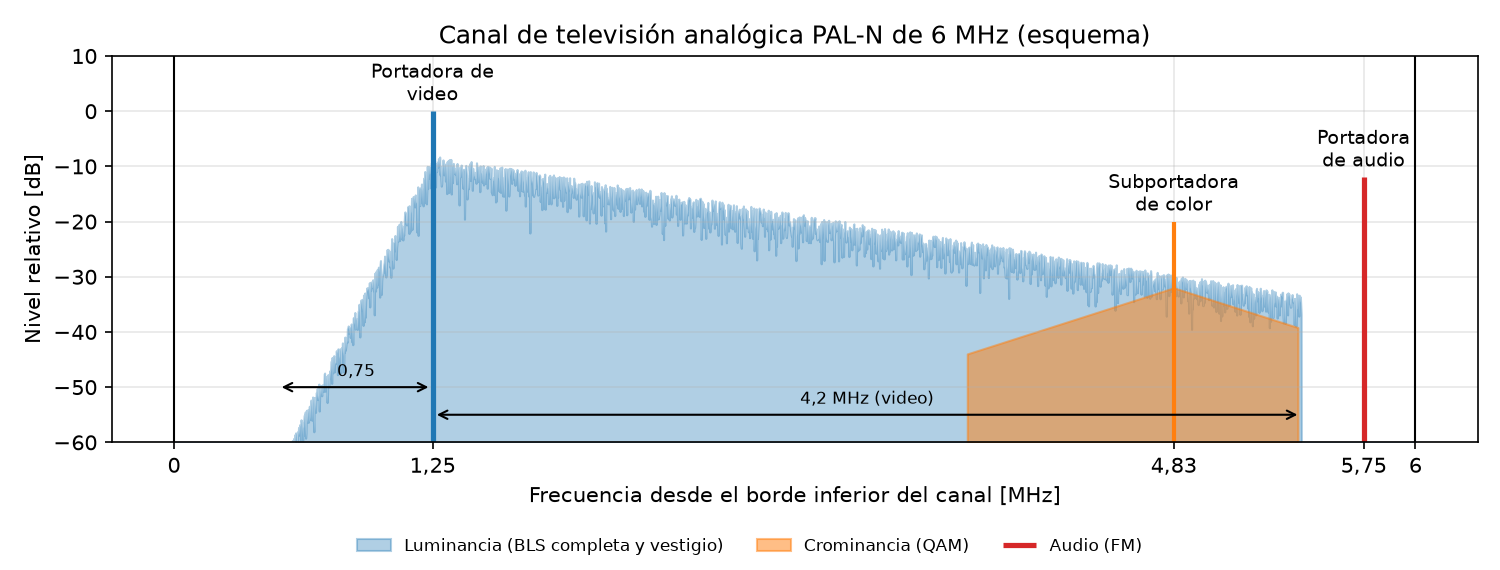
\includegraphics[width=\textwidth]{teoria/tv_pal_n.png}
    \caption{Espectro de un canal de televisión analógica PAL-N de $6 \, [MHz]$. Esquema propio a partir de la Rec. UIT-R BT.470 \cite{itu_bt470}.}
    \label{fig:tv_pal_n}
\end{figure}

\subsection{Mediciones}
\begin{table}[H]
    \centering
    \caption{Configuración del analizador y resultados para la señal de televisión analógica.}
    \label{tab:tv_resultados}
    \begin{tabular}{p{6.8cm} p{7.4cm}}
        \toprule
        \textbf{Parámetro} & \textbf{Valor} \\
        \midrule
        Canal y límites del canal & \pendiente{canal $N$, de $f_1$ a $f_2$ [MHz]} \\
        Frecuencia central / \textit{span} & \pendiente{} / \pendiente{$\approx 8 \, [MHz]$} \\
        Nivel de referencia / RBW / VBW & \pendiente{} \\
        Atenuación / preamplificación / unidad & \pendiente{} \\
        \midrule
        Portadora de video: frecuencia y nivel & \pendiente{} \\
        Subportadora de color: frecuencia y nivel & \pendiente{} \\
        Portadora de audio: frecuencia y nivel & \pendiente{} \\
        Relación audio/video & \pendiente{dB} \\
        Ancho de banda ocupado & \pendiente{MHz} \\
        \bottomrule
    \end{tabular}
\end{table}

\begin{figure}[H]
    \centering
    \pendiente{Captura del canal analógico (\texttt{Figuras/mediciones/tv\_analogica.png})}
    \caption{Espectro medido del canal de televisión analógica.}
    \label{fig:tv_medida}
\end{figure}

\subsection{Análisis}

\subsubsection*{Ancho de banda y banda lateral vestigial}
La señal ocupa unos $0{,}75 + 4{,}2 = 4{,}95 \, [MHz]$ de video, más el audio, dentro del canal de $6 \, [MHz]$. Con doble banda lateral, el video ocuparía $2 \times 4{,}2 = 8{,}4 \, [MHz]$ y no entraría en el canal. Con banda lateral única, en cambio, haría falta un filtro de corte abrupto justo en la portadora, imposible de construir sin distorsionar las bajas frecuencias del video, que son las de mayor energía (el nivel medio de la imagen y los sincronismos). La banda lateral vestigial es el compromiso entre ambas:
\begin{itemize}
    \item Se transmite la banda superior completa y un vestigio de la inferior, lo que permite un filtro de transmisión con una pendiente realizable.
    \item El receptor tiene un filtro de Nyquist, con una pendiente simétrica alrededor de la portadora: la suma de las dos bandas en la zona del vestigio reconstruye una respuesta plana.
    \item El receptor puede seguir usando un detector de envolvente.
\end{itemize}
\pendiente{Comparar con el ancho medido en la \autoref{fig:tv_medida}.}

\subsubsection*{Nivel del audio respecto del video}
La portadora de audio se transmite normalmente unos $10 \, [dB]$ por debajo del pico de la portadora de video. En la medición, el nivel de la portadora de video depende del contenido de la imagen, porque con modulación negativa una imagen clara reduce la amplitud media. Por eso la relación debe medirse con retención de máximos, para captar el nivel de los pulsos de sincronismo, que corresponden al pico de la envolvente, y con un RBW que contenga la portadora completa pero no las bandas laterales. \pendiente{Indicar la relación medida y las condiciones.}

\subsubsection*{Canales adyacentes}
\pendiente{Describir las señales detectadas en los canales vecinos.} El audio de un canal está a $0{,}25 \, [MHz]$ del borde superior y el vestigio del canal siguiente empieza $0{,}5 \, [MHz]$ por encima de ese borde, de modo que en una misma zona no se asignan canales adyacentes por aire. En las redes de cable, en cambio, se usan todos los canales contiguos, con niveles controlados.

\subsection{Síntesis}
En la televisión analógica PAL-N cada componente usa una modulación distinta dentro del mismo canal de $6 \, [MHz]$:
\begin{itemize}
    \item \underline{Video:} AM con banda lateral vestigial y modulación negativa.
    \item \underline{Color:} modulación en cuadratura de una subportadora en $3{,}58 \, [MHz]$, con alternancia de fase por línea, que ocupa la parte alta del espectro de luminancia sin interferirlo apreciablemente.
    \item \underline{Audio:} FM en una portadora $4{,}5 \, [MHz]$ por encima de la de video.
\end{itemize}
